\section{Funkcja falowa}

\subsection{Eksperyment z dwoma szczelinami}

Wobrażmy sobie ścianę z dwoma wąskimi otworami oraz drugą równoległą ścianę za nią, która nie ma żadnych otworów.
Teraz wyobraźmy sobie, że osoba strzela kulami we wszystkich kierunkach. Większość kul zatrzymuje się na pierwszej ścianie,
lecz część kul przechodzi przez otwory i trafia na drugą ścianę.
Jakiego obrazu spodziewamy się na drugiej ścianie? Spodziewamy się dwóch kropek, w miejscach odpowiadających otworom na pierwszej ścianie. To też obserwujemy.

\begin{figure}[H]
    \centering
    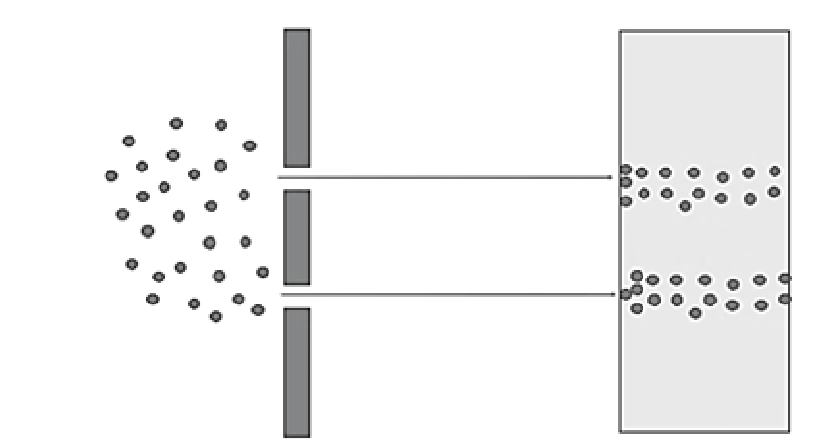
\includegraphics[width=0.5\textwidth]{szczeliny}
    \caption{Eksperyment z dwoma szczelinami. \textit{Źródło: Ranjbar, Vahid. (2023)}}
    \label{fig:szczeliny}
\end{figure}

\subsection{Eksperyment ze światłem}
W roku 1801 Thomas Young przeprowadził podobny eksperyment, ale przepuszczając przez szczeliny światło.
Przez dwie szczeliny przechodziła tak zwana fala płaska, poruszająca się w kierunku ekranu.
W sensie optyki klasycznej albo termodynamiki klasycznej, możemy powiedzieć, że przykładowo światło słoneczne jest taką falą płaską.
Ta fala płaska przechodzi przez szczeliny, a następnie dalej jako fala płaska przemieszcza się w kierunku oddalonego ekranu.

Co zobaczymy na ekranie? Na ekranie zobaczymy coś niespodziewanego - będzie to obraz interferencyjny.
\begin{figure}[H]
    \centering
    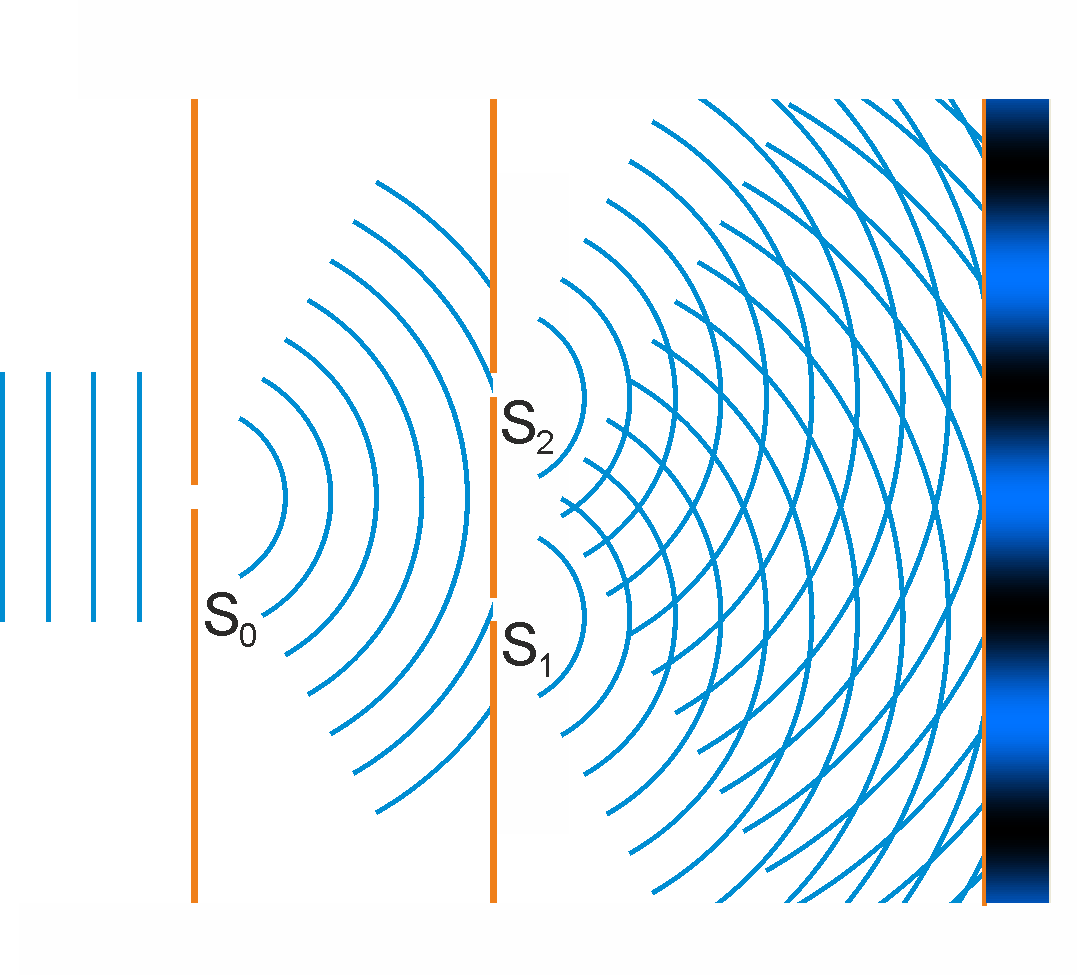
\includegraphics[width=0.5\textwidth]{szczeliny-fale}
    \caption{Eksperyment z dwoma szczelinami. \textit{Źródło: e-Fizyka, AGH}}
    \label{fig:szczeliny-fale}
\end{figure}

Zastanówmy się, w jaki sposób można opisać intensywności światła ukazujące się na ekranie.

Zacznijmy od amplitudy fali (amplitudy światła) - jest to wektor zależny od położenia w~przestrzeni oraz czasu:
\begin{equation*}
    A(\bar{r}, t)
\end{equation*}
Intensnywność światła $I$ można zapisać jako kwadrat amplitudy niezależnej od modułu:
\begin{equation*}
    I = |A|^2
\end{equation*}
Następnie pojawia się tak zwana zasada superpozycji. Aby obliczyć amplitudę całkowitą, musimy zsumować amplitudy fal pochodzących z obu szczelin (z obu źródeł):
\begin{equation*}
    \bar{A}(\bar{r}, t) = \bar{A}_1(\bar{r}, t) + \bar{A}_2(\bar{r}, t)
\end{equation*}

Intensywność całkowita będzie przybierać następującą postać:
\begin{equation*}
    I = |A_1|^2 + |A_2|^2 + A_1 A_2^* + A_1^* A_2
\end{equation*}

Człon $A_1 A_2^* + A_1^* A_2$ jest odpowiedzialny za interferencję. Obraz widoczny na ekranie jest spowodowany superpozycją fal pochodzących z obu szczelin.

\subsection{Proste zagadnienie}

Rozważmy najprostsze zagadnienie. W tym zagadnieniu podkreślamy, że odległość między szczelinami $d$ jest mała (dużo mniejsza niż odległość do ekranu $D$).
Na ekranie zaznaczamy pewien punkt $x$ oraz zaznaczamy odległości punktu $x$ od szczelin. Odległość $x$ od szczeliny $1$ wynosi $r_1$, a odległość $x$
od szczeliny $2$ wynosi $r_2$.

\begin{figure}[H]
    \centering
    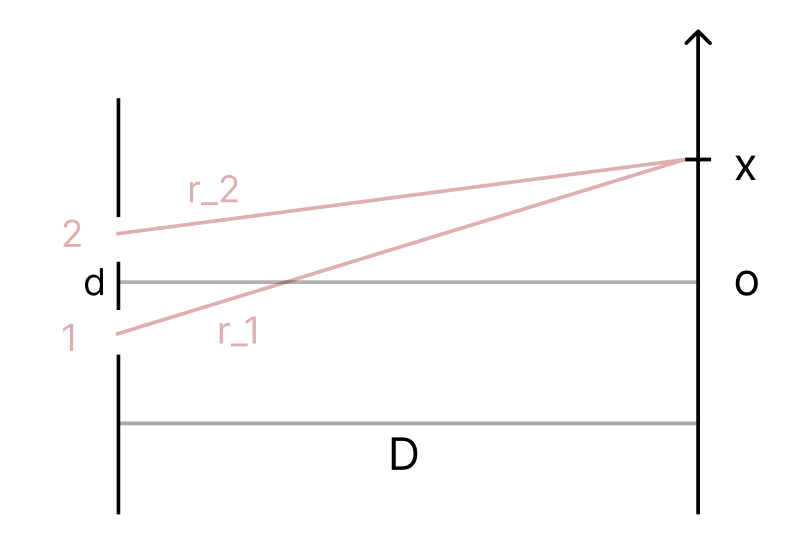
\includegraphics[width=0.5\textwidth]{prosty-eksperyment}
    \caption{Prosty eksperyment.}
    \label{fig:prosty-eksperyment}
\end{figure}

Rozważamy proste fale monochromatyczne, to znaczy amplitudy dla nich mają następującą postać:
\begin{equation*}
    A_1 = a_1 \exp[i(\omega t - \bar{k} \bar{r}_1 + \delta_1)]
\end{equation*}
\begin{equation*}
    A_2 = a_2 \exp[i(\omega t - \bar{k} \bar{r}_2 + \delta_2)]
\end{equation*}

Ponieważ mamy jedno źródło światła, możemy przyjąć, że $a_1 = a_2 = a$ i $\delta_1 = \delta_2 = 0$. 
Symbol $k$ oznacza wektor falowy, który ma kierunek fali. Zapisujemy go jako:
\begin{equation*}
    k = \frac{2\pi}{\lambda}
\end{equation*}
Wersor kierunku fali zapisujemy jako:
\begin{equation*}
    \frac{\bar{k}}{|k|}
\end{equation*}
Przechodzimy do geometrii. Chcemy zrozumieć, jaka będzie intensywność w punkcie $x$ na ekranie.

Wektory $\bar{k}_1$ i $\bar{k}_2$ będą równoległe do siebie, zatem możemy zapisać: $\bar{k}_1 = \bar{k}_2$.


Wyznaczamy $r_1^2$ i $r_2^2$:
\begin{equation*}
    r_1^2 = D^2 + \left(x + \frac{d}{2} \right)^2
\end{equation*}
\begin{equation*}
    r_2^2 = D^2 + \left(x - \frac{d}{2} \right)^2
\end{equation*}
Stąd:
\begin{equation*}
    r_1^2 - r_2^2 = 2xd
\end{equation*}
Ponieważ $r_1$ i $r_2$ są bardzo duże, a różnica między nimi jest mała, możemy zapisać:
\begin{equation*}
    r_1 - r_2 \approx \frac{xd}{D}
\end{equation*}
Intensywność końcowa:
\begin{align*}
    I &= \left(a\cdot e^{i\omega t}\right)^2 \cdot \left[e^{-ikr_1}+e^{-ikr_2}\right]^2 \\
    &= 2 a^2 \left(\cos{\left(kr_1-kr_2\right)}+1\right) \\
    &= 2 a^2 \left(1 + \cos{\left(k(r_1-r_2)\right)}\right) \\
    &= 2 a^2 \left(1 + \cos{\left(\frac{2\pi}{\lambda}\cdot\frac{xd}{D}\right)}\right) = I(x)
\end{align*}

Pytanie - dla jakich $x$ będzie maksymalna intensywność?
Aby znaleźć maksimum, obliczamy pochodną $I(x)$ i przyrównujemy do zera - wartość w zerze będzie albo maksimum, albo minimum.
Chcemy zatem, aby argument cosinusa przyjmował wartość $1$. Będzie to dla $2k\pi$, $k=0,1,2,3,\ldots$. Przyrównując:
\begin{equation*}
    \frac{2\pi}{\lambda} \frac{xd}{D} = 2k\pi
\end{equation*}
Rozwiązując dla $x$ otrzymujemy:
\begin{equation*}
    x_{max} = k \frac{\lambda D}{d}
\end{equation*}
W ten sposób możemy wytłumaczyć obraz interferencyjny - pojawiają się punkty o maksymalnej intensywności
rozłożone wzdłuż osi $x$, a odległość między kolejnymi punktami wynosi $\frac{\lambda D}{d}$.

\subsection{Ciało czarne}

\textbf{Ciało czarne}, gdy jest zimne, pochłania wszystkie barwy (światło), ale gdy jest bardzo podgrzane, to świeci na biało.
Słońce jest ciałem czarnym.

\subsection{Światło jako fala}
Przykład dla dwóch szczelin:
\[
A(\vec{r}, t) = A_1(\vec{r}, t) + A_2(\vec{r}, t)
\]
gdzie $A_1(\vec{r}, t)$ i $A_2(\vec{r}, t)$ są amplitudami fal przechodzących przez każdą ze szczelin.

Natężenie światła wyraża się wzorem:
\[
I(\vec{r}, t) = |A(\vec{r}, t)|^2
\]
co oznacza, że natężenie światła w danym punkcie jest proporcjonalne do kwadratu amplitudy fali w tym punkcie.

\subsection{Elektron jako fala}
W mechanice kwantowej elektron $e^-$ jest traktowany jako fala, co jest formalnie określone poprzez funkcję falową. 

Funkcja falowa $\Psi(x,y,z,t)$ opisuje stan elektronu w trójwymiarowej przestrzeni oraz w~czasie. Dla swobodnego elektronu można przyjąć:
\[
\Psi(x,y,z,t) \sim A(\vec{r}, t)
\]
gdzie $A(\vec{r},t)$ jest amplitudą fali elektronowej.

Kwadrat modułu funkcji falowej $|\Psi(\Sigma, t)|^2$ jest \textbf{prawdopodobieństwem} (gęstością prawdopodobieństwa) znalezienia cząstki w danym obszarze przestrzeni w danym czasie.
Przy czym: 0 - brak cząstki, 1 - jakaś cząstka została zarejestrowana. Można go traktować jako ,,intensywność'' fali elektronowej.

Obowiązuje zasada superpozycji (tak jak dla światła).
Zatem jeżeli mamy dwie funkcje falowe, $\Psi_A$ i $\Psi_B$, możemy je zsumować, otrzymując nową funkcję falową, będącą superpozycją tych funkcji.
\[
\Psi = \Psi_A + \Psi_B \quad P \sim |\Psi_A + \Psi_B|^2 \neq |\Psi_A|^2 + |\Psi_B|^2
\]
Prawdopodobieństwo znalezienia elektronu w danym miejscu jest proporcjonalne do kwadratu modułu sumy funkcji falowych,
co oznacza, że prawdopodobieństwo znalezienia elektronu w danym miejscu jest zależne od interferencji fal $\Psi_A$ i $\Psi_B$.

\subsection{Interpretacja fali elektronowej}
Mamy jeden elektron, tzn. mamy jeden sygnał, że w danym czasie go zaobserwujemy.
Całkowite prawdopodobieństwo, że w całej przestrzeni znajdziemy elektron musi być równe 1.
Dlatego funkcja falowa musi być znormalizowana, zatem:
\[
\int |\Psi(\vec{r}, t)|^2 d\vec{r} = 1 = \int \Psi \Psi^* d\vec{r}
\]
Wyrażenie może być ciągłe (np. dla fali) lub dyskretne.
Szukamy znormalizowanej funkcji $\Psi$, tzn. $\Psi$ dzielimy/mnożymy, aby uzyskać 1.

Wróćmy do superpozycji dwóch funkcji falowych. Ogólna funkcja falowa może być liniową kombinacją dwóch funkcji falowych, gdzie $c_1$ i $c_2$ są współczynnikami.
Każda funkcja falowa może być wyrażona w postaci zespolonej, z amplitudą $|\Psi_i|$ oraz fazą $\delta_i$.
Stąd moduł kwadratu funkcji falowej $|\Psi|^2$ daje się rozwinąć do postaci:
\begin{align*}
\Psi &= c_1 \Psi_1 + c_2 \Psi_2\\
\Psi_1 &= |\Psi_1| e^{i \delta_1}\\
\Psi_2 &= |\Psi_2| e^{i \delta_2}\\
|\Psi|^2 &= c_1^2 |\Psi_1|^2 + c_2^2 |\Psi_2|^2 + 2 \Re (c_1 c_2^* |\Psi_1| |\Psi_2| e^{i (\delta_1 - \delta_2)})
\end{align*}
Ten wzór uwzględnia zarówno intensywności poszczególnych fal, jak i interferencję między nimi. Człon odpowiedzialny za interferencję ma postać:
\begin{equation*}
    2 \Re \left[ c_1 c_2^* |\Psi_1| |\Psi_2| e^{i (\delta_1 - \delta_2)} \right]
\end{equation*}

\subsection{Fala de Broglie'a}
\[
E = h\nu, \quad E = \hbar \omega
\]
\[
p = \frac{h}{\lambda}, \quad p = \hbar k, \quad k = \frac{2\pi}{\lambda}
\]
Gdzie:
\begin{itemize}
    \item $E$ to energia,
    \item $\nu$ to częstotliwość,
    \item $\lambda$ to długość fali,
    \item $p$ to pęd cząstki,
    \item $k$ jest wektorem, który opisuje kierunek i długość fali.
\end{itemize}

\subsection{Fala płaska}
Równanie fali płaskiej:
\[
\Psi(x,y,z,t) = A \exp \left( i \left( kx - \omega t \right) \right)
\]
Można również zapisać jako:
\[
\Psi = A \exp \left( \frac{i}{\hbar} (p_x x - E(p_x) t) \right)
\]
\begin{itemize}
    \item W zależności od położenia rzeczywista część to cosinus i to jest zwykła fala.
    \item Najprostszy obiekt jaki możemy mieć.
    \item Stojąca fala może się zdarzyć, że nie będzie płaska.
    \item Stojąca jednowymiarowa fala jest płaska.
    \item Kierunek przestrzeni może być dowolny, nie musi to być $x$.
\end{itemize}

Dla trzech wymiarów zapisujemy:
\[
\Psi(\vec{r}, t) = A \exp \left( \frac{i}{\hbar} (\vec{p} \cdot \vec{r} - E(p) t) \right)
\]

Pęd jest opisany jako:
\[
\vec{p} \equiv \hbar \vec{k}
\]

Dużym problemem jest całka po całej przestrzeni, bo jest nieskończona.

$\partial_x$: $-i\hbar \frac{\partial}{\partial x} \Psi = p_x \Psi$,

$\partial_t$: $i\hbar \frac{\partial}{\partial t} \Psi = E \Psi$

Operator pędu:
\[
\vec{P}_0 = -i\hbar \vec{\nabla}
\]

\subsection{Pakiety falowe}
Zamiast jednej fali zbiór fal (jesteśmy w jednym wymiarze):
\[
\Psi(x,t) = (2\pi\hbar)^{-1/2} \int_{-\infty}^{+\infty} \phi(p_x) e^{\frac{i}{\hbar} (p_x x - E(p_x) t)} dp_x
\]
Wyrażenie pod całką to \textbf{fala płaska}, a $\phi(p_x)$ to funkcja określająca pakiet falowy.

Rozważmy $t = 0$, wtedy funkcję falową w przestrzeni położenia ma postać:
\[
\Psi(x,0) = (2\pi\hbar)^{-1/2} \int_{-\infty}^{+\infty} \phi(p_x) e^{\frac{i}{\hbar} p_x x} dp_x
\]

Funkcję falową w przestrzeni pędu możemy zapisać jako:
\[
\phi(p_x) = (2\pi\hbar)^{-1/2} \int e^{-\frac{i}{\hbar} p_x x} \Psi(x) dx
\]
Jest to transformata Fouriera.

Niech $\Psi'(x) = (2\pi\hbar)^{-1/2} e^{\frac{i}{\hbar} p_x x}$, wtedy:
\begin{align*}
\phi(p_x) &= (2\pi\hbar)^{-1/2} \int e^\frac{-ip_x x}{\hbar} \cdot e^\frac{ip'_x x}{\hbar} dx \\
&= (2\pi\hbar)^{-1/2} \int e^\frac{i(p'_x - p_x) x}{\hbar} dx \\
&= \delta(p'_x - p_x)
\end{align*}

Fala na przykład po wrzuceniu kamienia do wody to superpozycja różnych częstości.

\[
\int |\delta(p'_x - p_x)|^2 dp_x = \delta(0)
\]

\subsection{Pakiet Gaussowski}
Funkcja $\phi(p_x)$ dla pakietu Gaussowskiego ma postać:
\[
\phi(p_x) = C \exp \left( -\frac{(p_x - p_0)^2}{2 (\Delta p_x)^2} \right)
\]

gdzie $\Delta p_x$ oznacza szerokość pakietu, a $p_0$ to środek pakietu.

\[
\int |\phi(p_x)|^2 dp_x = 1 = |C|^2 \pi^{1/2} (\Delta p_x)
\]
Stąd:
\[
C = \pi^{-\frac{1}{4}} \frac{1}{\sqrt{\Delta p_x}}
\]

\[
\int e^{-\alpha/\mu^2} e^{-\beta \mu^2} d\mu = \left(\frac{\pi}{\alpha}\right)^\frac{1/2} \exp{\frac{\beta^2}{4\alpha}}
\]

\begin{align*}
\Psi(x) &= (2\pi\hbar)^{-1/2} \int e^{\frac{i}{\hbar} (p_x x - E(p_x) t)} \phi(p_x) dp_x \\
&= \cdots \\
&= \pi^{-1/4} \hbar^{-1/2} (\Delta p_x)^{-1/2} e^{\frac{ip_0 x}{\hbar} e^{-(\Delta p_x)^2 x^2}{2\hbar^2}}
\end{align*}

\[
(\frac{(\Delta p_x)^2}{\hbar^2}) = \frac{1}{(\Delta x)^2} \quad \Delta x \Delta p_x = \hbar
\]
\begin{itemize}
    \item Jeśli pakiet jest dobrze zlokalizowany (wąski) w przestrzeni, to jest źle zlokalizowany w przestrzeni pędu.
    \item Jeśli jest nieskończenie szeroki to nie znajdziemy elektronu.
\end{itemize}

\subsection{Ewolucja w czasie}

Energia wyrażona przez pęd:
\[
E = \frac{p_x^2}{2m}
\]

Funkcja falowa w czasie:
\begin{align*}
\Psi(x,t) &= \left(2\pi\hbar \right)^{-1/2} \int e^{i\frac{p_x x - E(p_x)t}{\hbar}} \phi(p_x) dp_x \\
&= \pi^{-\frac{1}{4}}\left[\frac{\frac{\Delta p x}{\hbar}}{1+i\frac{(\Delta p_x)^2 t}{m\hbar}}\right] \exp\left[\frac{\frac{ip_0 x}{\hbar}-\left(\frac{\Delta p_x}{\hbar}\right)^2\frac{x^2}{2}-\frac{ip_0 t}{2x\hbar}}{1+i(\Delta p_x)^2 \frac{t}{m\hbar}}\right]
\end{align*}

\[
|\Psi(x,t)|^2 = \pi^{-\frac{1}{2}}\left[\frac{\frac{\Delta p x}{\hbar}}{\left[1+i\frac{(\Delta p_x)^4 t^2}{m^2\hbar^2}\right]^{\frac{1}{2}}}\right] \exp\left[\frac{-\left(\frac{\Delta p_x}{\hbar}\right)^2(x-V_gt)^2}{1+\frac{(\Delta p_x)^4 t^4}{m^2\hbar^2}}\right]
\]

Prędkość grupowa:
\[
V_g = \frac{p_0}{m}
\]
Rozważamy szczególny przypadek.
\[
\Delta x (t) = \frac{\hbar}{\Delta p_x} \underbrace{\left[1 + \frac{(\Delta p_x)^4}{m^2\hbar^2}t^2\right]^{1/2}}_{B}
\]
Zawsze $B \geq 1$.
\[
\Delta x \Delta p = \hbar B
\]

Nierówność Heisenberga:
\[
\Delta x \Delta p \geq \hbar
\]

To jest grube przybliżenie, ponieważ rzeczywistość wymaga bardziej dokładnych obliczeń.

Interpretacja $x$ to błąd wymiaru.
\[
\Delta y \Delta p_y \geq \hbar
\]
\[
\Delta z \Delta p_z \geq \hbar
\]

\subsection{Para czas/energia}
Transformata Fouriera:
\[
\begin{cases}
\Psi(t) = \frac{1}{\sqrt{2\pi}} \int G(\omega) e^{-i\omega t} d\omega\\
G(\omega) = \frac{1}{\sqrt{2\pi}} \int \Psi(t) e^{i\omega t} dt
\end{cases}
\]

Stąd
\[
\Delta \omega \Delta t \geq 1
\]

Związek nieoznaczoności:
\[
\Delta E \Delta t \geq \hbar
\]

Zależność energii od częstotliwości:
\[
E = \hbar \omega
\]

\subsection{Równanie Schrödingera}

\textbf{Motywacja}: chcemy znaleźć równanie, które będzie opisywało ewolucję fali.

\[
\begin{cases}
    \Psi_1 \text{ -- rozwiązanie} \\
    \Psi_2 \text{ -- rozwiązanie}
\end{cases} \Rightarrow c_1 \Psi_1 + c_2 \Psi_2 \text{ -- rozwiązanie}
\]
Rozwiązanie równania Schrödingera jest liniowe. $\Psi$ musi posiadać pierwszą pochodną.

Fala płaska:
\[
\Psi(x,t) = A e^{\frac{i(px x - Et)}{\hbar}}
\]

$\frac{\partial}{\partial x}$ $-i \hbar \frac{\partial}{\partial x} \Psi = p_x \Psi \xRightarrow{\frac{\partial}{\partial x}} \frac{\partial^2\Psi}{\partial x^2} = -\frac{p^2}{\hbar^2} \Psi = -\frac{2mE}{\hbar^2} \Psi$

$\frac{\partial}{\partial t}$ $\frac{\partial\Psi}{\partial t} = \frac{-iE\Psi}{\hbar}$

\[
-i\hbar \frac{\partial}{\partial t} \Psi(x, t) = -\frac{-\hbar^2}{2m} \frac{\partial^2}{\partial x^2} \Psi(x, t)
\]

Interpretacja:
\[
-i\hbar \frac{\partial}{\partial x} \sim p_x \Rightarrow \frac{-\hbar^2}{2m} \frac{\partial^2}{\partial x^2} \sim E_{\text{kin}}
\]

Gdy dodamy potencjał $V(x,t)$:
\[
-i\hbar \frac{\partial}{\partial t} \Psi(x,t) = \left[ -\frac{\hbar^2}{2m} \frac{\partial^2}{\partial x^2} + V(x,t) \right] \Psi(x,t)
\]
Gdy $V(x,t) = 0$ to mamy rozwiązanie.
W trzech wymiarach:
\[
i\hbar \frac{\partial}{\partial t} \Psi(\vec{r},t) = \left[ -\frac{\hbar^2}{2m} \nabla^2 + V(\vec{r},t) \right] \Psi(\vec{r},t)
\]
Jest to równanie Schrödingera.
